\documentclass{beamer}
\usetheme{Warsaw}

\usepackage[utf8]{inputenc}
\usepackage{fancybox}
\usepackage{multimedia} 
\usepackage{subfig}
\usepackage{amsmath}
\usepackage{hyperref}
\hypersetup{
    colorlinks=true,     
    urlcolor=blue
}
\usepackage[all]{xy}
\begin{document}


\title[Stochastik] % (optional, only for long titles)
{Stochastik für Informatiker
\\
\includegraphics[scale=0.5]{img/craps}
}
\subtitle{}
\author[Dr. Johannes Riesterer] % (optional, for multiple authors)
{Dr.  rer. nat. Johannes Riesterer}

\date[KPT 2004] % (optional)
{}

\subject{Stochastik}


\frame{\titlepage}





\begin{frame}
    \frametitle{Erwartungswert}
\framesubtitle{}
\begin{block}{Erwartungswert}
Eine reelle Zufallsvariable ist integrierbar und ihr Erwartungswert wird definiert durch
$$ \mathbb{E} (X) := \int_{\Omega} X \; dP \; .$$
\end{block}
 \end{frame}


\begin{frame}
    \frametitle{Erwartungswert}
\framesubtitle{}
\begin{block}{Erwartungswert}
Ist $(\Omega, \mathcal{A}, P)$ ein diskreter Wahrscheinlichkeitsraum und $X :\Omega \to \mathbb{R}$ eine eindimensionale reelle Zufallsvariable, so ist
$$ \mathbb{E} (X) = \sum_{\omega \in \Omega}  X(\omega) \cdot P(\omega)$$
\end{block}
 \end{frame}


\begin{frame}
    \frametitle{Erwartungswert}
\framesubtitle{}
\begin{block}{Transformationsformel}
Für eine reelle Zufallsvariable $X: \Omega \to \mathbb{R}^n$ und eine integrierbare Funktion $g:  \mathbb{R}^n \to \mathbb{R}$ gilt
$$ \mathbb{E} (g \circ X) := \int_{\Omega} g \circ X \; dP = \int_{\mathbb{R}^n}  g \; dP_X \;. $$
Ist insbesondere $f(x) : \mathbb{R}^n \to \mathbb{R}$ eine Dichte für $P_X$ , so ist  
$$\mathbb{E} (X) =  \int_{\mathbb{R}^n} x \cdot f(x) \; d\mu$$ das Lebesgue-Integral der Funktion $x \cdot f(x)$.
\end{block}
 \end{frame}


\begin{frame}
    \frametitle{Erwartungswert}
\framesubtitle{}
\begin{block}{Transformationsformel}
Für $g = 1_A$ mit $A \in \mathcal{B}(\mathbb{R}^n)$ ist
\begin{align*}
& \int 1_A \; dP_X = P_X(A) = P(X^{-1} (A)) = \int 1_{X^{-1}(A)} \; dP \\
&= \int 1_{A} \circ X \; dP
\end{align*}
Für eine Treppenfunktion $g= \sum_{i= 1}^n c_i 1_{A_i} $folgt das Ergebnis aus der Linearität des Integrals  für Treppenfunktionen. Für integrierbares $g$ folgt das Resultat mit Hilfe von Konvergenzsätzen für das  Integral.
\end{block}
 \end{frame}

\begin{frame}
    \frametitle{Erwartungswert}
\framesubtitle{}
\begin{block}{Beispiel}
$\Omega = \{ \text{Kopf},\text{Zahl}\}$, $P(\text{Kopf}) = P(\text{Zahl}) = \frac{1}{2}$, $X(\text{Kopf}) = 0,  X(\text{Zahl}) = 1$ 
\begin{align*}
& \mathbb{E}(X)  = 0 \cdot P(X^{-1}(0) ) + 1 \cdot P(X^{-1}(1)) \\
& =0  \cdot P(\text{Kopf}) + 1 \cdot P(\text{Zahl}) = \frac{1}{2}  
\end{align*}
\end{block}
 \end{frame}



\begin{frame}
    \frametitle{Erwartungswert}
\framesubtitle{}
\begin{block}{Beispiel}
Sei $X \sim \mathcal{N}(\mu, \sigma^2)$.
\begin{align*}
\mathbb{E}(X) & := \int_{\mathbb{R}}  x \cdot  \frac 1{\sigma \sqrt{2\pi}}e^{- \frac {1}{2 } (\frac{x- \mu}{ \sigma})^2} \; dx  \\
&= \int_{\mathbb{R}}  (y + \mu) \cdot  \frac 1{\sigma \sqrt{2\pi}}e^{- \frac {1}{2 \sigma^2} y^2} \; dy \\
 &  = \mu  \int_{\mathbb{R}}      \frac 1{\sigma \sqrt{2\pi}}e^{- \frac {1}{2 \sigma^2} y^2} \; dy  + \int_{\mathbb{R}}  y  \cdot  \frac 1{\sigma \sqrt{2\pi}}e^{- \frac {1}{2 \sigma^2} y^2} \; dy = \mu
\end{align*}
\end{block}
\begin{figure}[htp]
      \centering
    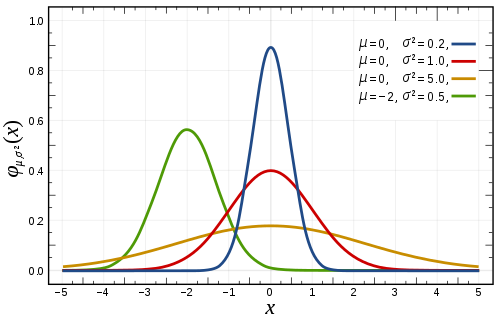
\includegraphics[width=0.46\textwidth]{img/normal}
      \caption{Quelle: Wikipedia}
\end{figure}
 \end{frame}




\begin{frame}
    \frametitle{Erwartungswert}
\framesubtitle{}
\begin{block}{Eigenschaften}
Sind $X,Y : \Omega \to \mathbb{R}^n$   reelle, integrierbare  Zufallsvariablen und $a,b \in \mathbb{R}$ konstant, so gilt:
\begin{align*}
& \mathbb{E}(a \cdot X + b \cdot Y) = a \cdot \mathbb{E}(X) + b \cdot \mathbb{E}(Y) \\
& X(x) \leq Y(x) \;  \forall x \in \Omega \Rightarrow \mathbb{E}(X) \leq \mathbb{E}(Y) \\
& X ,Y \text{ stoch. unabhängig} \Rightarrow   \mathbb{E}(X \cdot Y) =  \mathbb{E}(X) \cdot  \mathbb{E}(Y) \\
& \mathbb{E} (1_A) = P (A)
\end{align*}
\end{block}
 \end{frame}


\begin{frame}
    \frametitle{Erwartungswert}
\framesubtitle{}
\begin{block}{Markov Ungleichung}
Sei $Y : \Omega \to \mathbb{R}$  eine  reelle, integrierbare  Zufallsvariable und $f : [0, \infty) \to [0, \infty)$ monoton wachsend.
Dann gilt für alle $\epsilon > 0$ mit $f(\epsilon) > 0$
\begin{align*}
P (|Y |  \geq \epsilon) \leq \frac{\mathbb{E} (f \circ |Y|)}{f(\epsilon)}
\end{align*}
\end{block}
\begin{block}{Beweis}
Da $f(\epsilon) 1_{\{ |Y| \geq  \epsilon \} } \leq f \circ |Y|$ folgt
\begin{align*}
f(\epsilon) P(|Y| \geq \epsilon) = & f(\epsilon) \mathbb{E}(1_{\{ |Y| \geq  \epsilon \} }) = \mathbb{E}( f(\epsilon) 1_{\{ |Y| \geq  \epsilon \} }) \\
\leq & \mathbb{E}( f \circ |Y|)
\end{align*}
\end{block}
 \end{frame}


\begin{frame}
    \frametitle{Erwartungswert}
\framesubtitle{}
\begin{block}{Varianz}
Für eine reelle Zufallsvariable ist die Varianz definiert durch
$$ \mathbb{V} (X) :=  \mathbb{E}( (X - \mathbb{E}(X))^2) \; .$$
\end{block}
\begin{block}{Verschiebungssatz}

\begin{align*}
 \mathbb{V}(X) & = \mathbb{E}(X^2 - 2X \mathbb{E}(X) + \mathbb{E}(X)^2) = \mathbb{E}(X^2) - 2 \mathbb{E}(X)^2 +  \mathbb{E}(X)^2 \\
& =  \mathbb{E}(X^2) -  \mathbb{E}(X)^2 \\
\end{align*}
\end{block}
 \end{frame}


\begin{frame}
    \frametitle{Erwartungswert}
\framesubtitle{}
\begin{block}{Beispiel}
Sei $X \sim \mathcal{N}(\mu, \sigma^2)$.
\begin{align*}
&\mathbb{V} (X) =  \frac{1}{\sqrt{2 \pi}} \int_{- \infty}^{\infty} x^2 e^{- \frac{x^2}{2}} \; dx =   \frac{1}{\sqrt{2 \pi}} \int_{- \infty}^{\infty} x (xe^{- \frac{x^2}{2}}) \; dx \\
& =  \frac{1}{\sqrt{2 \pi}} \biggl (\biggl [ x (e^{- \frac{x^2}{2}}) \biggr]_{- \infty}^{\infty}   - \int_{- \infty}^{\infty}  - e^{- \frac{x^2}{2}} \; dx  \biggr) = 0 + 1 = 1\\
\end{align*}
\href{https://de.wikipedia.org/wiki/Partielle_Integration}{LINK: Partielle Integration}. Mit "Verschiebungstrick"
$\Rightarrow \mathbb{V}(X) = \sigma^2$.
\end{block}
 \end{frame}


\begin{frame}
    \frametitle{Erwartungswert}
\framesubtitle{}
\begin{block}{Tschebyscheff-Ungleichung}
Für eine reelle, integrierbare und quadratintegrierbare  Zufallsvariable $Y : \Omega \to \mathbb{R}$  gilt:
\begin{align*}
P (|Y  - \mathbb{E} (Y)|  \geq \epsilon) \leq \frac{\mathbb{V} (Y)}{ \epsilon^2} 
\end{align*}
\end{block}
\begin{block}{Beweis}
Folgt direkt aus der Markov-Ungleichung mit $Y' = Y -\mathbb{E}(Y)$ und $f(x) = x^2$
\end{block}
 \end{frame}


\begin{frame}
    \frametitle{Highlight}
\framesubtitle{}
\begin{figure}[htp]
      \centering
    
\includegraphics[width=0.9\textwidth]{img/firework}
\end{figure}
 \end{frame}


\begin{frame}
    \frametitle{Erwartungswert}
\framesubtitle{}
\begin{block}{Schwaches Gesetz der großen Zahlen}
Seien $X_i : \Omega \to \mathbb{R}$ unabhängige, reelle Zufallsvariablen (uid, iid(englisch)) mit $\mathbb{E}(X_i) = \mu < \infty$ und $\mathbb{V}(X_i) = \sigma < \infty$, dann gilt
\begin{align*}
P \bigl  ( \bigl | \frac{1}{n} \sum_{i=1}^{n} X_i - \mu \bigr |  \geq \epsilon \bigr) \leq \frac{\sigma}{ n \cdot \epsilon^2} \; \; \underset{n \to \infty}{\longrightarrow} 0
\end{align*}
(stochastische Konvergenz). 
\end{block}
 \end{frame}


\begin{frame}
    \frametitle{Erwartungswert}
\framesubtitle{}
\begin{block}{Beweis}
Mit $Y_n =  \frac{1}{n} \sum_{i=1}^{n}  X_i - \mu$ ist $\mathbb{E}(Y_n) =  \frac{1}{n} \sum_{i=1}^{n} \mathbb{E}( X_i - \mu) = 0$ und 
$\mathbb{V}(Y_n) =  \frac{1}{n^2} \sum_{i=1}^{n} \mathbb{V}( X_i ) = \frac{\sigma}{n}$. Aus der Tschebyscheff-Ungleichung folgt die Behauptung.
\end{block}
 \end{frame}


\begin{frame}
    \frametitle{Erwartungswert}
\framesubtitle{}

\begin{figure}[htp]
      \centering
    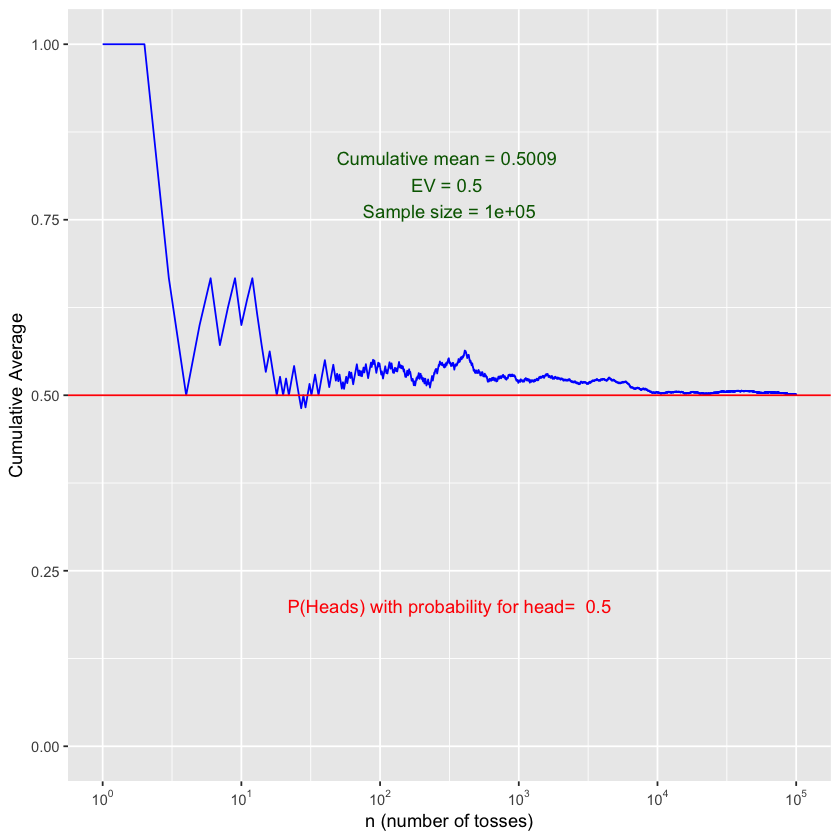
\includegraphics[width=0.86\textwidth]{img/sgdz}
      \caption{Quelle: Wikipedia}
\end{figure}
 \end{frame}



\end{document}
